\documentclass[10pt]{article}

\setlength{\oddsidemargin}{0.in}
\setlength{\textwidth}{6.5in}
\setlength{\topmargin}{0.in}
\setlength{\textheight}{8.5in}

%usepackage{hyperref}

\usepackage[pdftex]{graphicx}
\usepackage{url}
%\usepackage{chicago}
\usepackage{amsmath}
\usepackage{moreverb}
\usepackage{draftcopy}
\usepackage{multicol}
\usepackage{boxedminipage}
\usepackage{titlesec}
\usepackage{enumitem}
\usepackage{listings}
\usepackage{textcomp}


\RequirePackage{fancyhdr}
\RequirePackage[colorlinks]{hyperref}


\RequirePackage{fancyvrb}
\DefineVerbatimEnvironment{code}{verbatim}{fontsize=\small}

\RequirePackage{color}
%%% Find colors: http://en.wikipedia.org/wiki/List_of_colors
\definecolor{seagreen}{rgb}{0.18, 0.55, 0.34}
\definecolor{orangy}{cmyk}{0.0, 0.58, 0.100, 0.10}
\definecolor{saffron}{rgb}{0.96, 0.77, 0.19}
\definecolor{carmine}{rgb}{0.59, 0.0, 0.09}
\definecolor{chocolate}{rgb}{0.48, 0.25, 0.0}
\definecolor{darkraspberry}{rgb}{0.53, 0.15, 0.34}
\definecolor{electricindigo}{rgb}{0.44, 0.0, 1.00}
\definecolor{oldmauve}{rgb}{0.40, 0.19, 0.28}
\definecolor{blue-violet}{rgb}{0.54, 0.17, 0.89}
\definecolor{blue(pigment)}{rgb}{0.2, 0.2, 0.6}


\def\bookauthor{Dave Doolin}
\def\booklongtitle{PanzerBlitz Rules - Classic and House}
\def\wwkeywords{panzerblitz}
\def\wwsubject{tactical armored warfare}
\def\wwslug{mtngrown}

\hypersetup{%
 pdfauthor={\bookauthor},
 pdftitle={\booklongtitle},
 pdfkeywords={\wwkeywords},
 pdfsubject={\wwsubject},
 urlcolor=cyan,
 pdfdisplaydoctitle=true,
 pdfcreator={Website In A Weekend},
 pdfproducer={\LaTeX},
 baseurl={http://website-in-a-weekend.net/wiaw-whitepapers/\wwslug},
 breaklinks=false,
}

\title{Final Frontier Rules of Play}

\begin{document}

\maketitle


\tableofcontents


\begin{multicols}{2}

\section{Introduction}
\section{Game Components}

Most wargame rules have an counter images illustrating the meaning of values,
abbreviations and symbols on the counters. The Final Frontier does not! In a
spirit of contribution, here is an illustration of a counter, with the associated
explanation.

\begin{center}
  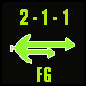
\includegraphics[width=100pt]{../../source/images/final-frontier-frigate.pdf}
\end{center}

\begin{itemize}
  \item ``FG'' stands for Frigate.
  \item The top row of numbers are ordered by Beam - Missile - Damage value.
  \item Any bottom number would be a surface combat value.
\end{itemize}

\section{Preparation For Play}
\section{Sequence Of Play}

Before each turn, advance the planets according to the Turn Track.

\begin{enumerate}
  \item Economics phase
  \item Space movement phase
  \item Space combat phase
  \item Space-surface interaction
  \item Surface combat
  \item Repeat for each player
\end{enumerate}

\section{Planets}
\section{Economics}


The economics phase is pretty simple. The complexity is induced
by the unclear explanation of the single entry bookkeeping ledger
supplied with the game.

Some hints:

* The ``income'' column is the total from all resources coming in from mines
and colonies. This number is entered first.

* The GNP is updated by adding the income to the previous turn's GNP.

* The ``Total'' column tracks the Build Points, which are best recorded
as an explicit sum of the current Build Point allotment cross-referenced
from GNP and NI, and the remainder BPs from the previous turn. For example,
suppose 1 BP left over and 3 are allotted. Record this in the ``Total'' column
as ``3 + 1'' instead of ``4.''.

\section{Political Events}
\subsection{National Interest Level}
\subsection{Colonization}

\section{Space Movement}

\section{Space Combat}

\section{Space-Surface Interaction}

\section{Surface Combat}

\section{Earth}

\section{Random Events}

\section{Victory Conditions}

\section{Designer's Notes}

\section{Game Credits}


\section{FAQs and more}

\subsection{National Interest Level}

\begin{itemize}
  \item NI never decreases.
  \item NI increases one step when the the population level of the the largest
    population counter (mine or colony) increases one step. See Section 7.2.
  \item Emplacing the first mine does not increase the NI.
  \item (House rule) The NI is increased when the colony is emplaced, not when
    it is built. This would be a good question for the forums.
\end{itemize}
\section{Summary}

\end{multicols}

\appendix

\section{Player aids}

\subsection{A better ledger}

The ledger which ships with the game is confusing, as it tracks GNP and
Build Points in the same rows, without clearly explaning how the columns
should be used. Compounding this is the problem with any single entry system,
how best to carry balances forward.

\subsection{Status record}

Final Frontier lends itself to solo play, and even better, lends itself
to play over time. The game system is simple enough to keep a record of
which pieces are in play, and what their status is, with a handy status
record.

The status record also records the position on the planets.

\subsection{Counter re-creation}

The counters as shipped are 7/16" square. I'm ``re-creating'' a few of the
counters for game play aid using Inkscape, and saving in SVG format.

{\tt DISPLAY= inkscape final-frontier-frigate.svg --export-pdf=final-frontier-frigate.pdf}

Some notes on the ship counters:

\begin{itemize}
  \item The font, evidently, is Compacta, but not bold. That said, Compacta Bold
    is a pretty close fit.
  \item For a nominal 5/8" counter, set the numbers at the top to 12 pt, the letters
    denoting ship type to 11 pt.
  \item With Inkscape, the font stroke should be set to zero, using the fill color to
    draw out the glyphs.
  \item On the ship outlines, set the stroke color to white, which provides a subtle pop
    to the silhouette.
  \item The stroke width on the ships is ???
\end{itemize}

The colors can be approximated using RGB values:

\begin{itemize}
    \item Chartreuse:
    \item Magenta:
    \item Cyan:
    \item Yellow:
\end{itemize}

\end{document}
